\documentclass[11pt]{amsbook}
\usepackage[turkish]{babel}

\usepackage{../Ceyhun}
\usepackage{../amsTurkish}


\begin{document}
	\hPage{ceyhun-204}
	\begin{figure}[h!]
		\begin{minipage}{0.5\textwidth}
			\centering
			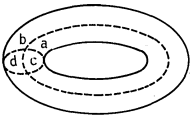
\includegraphics[width=.7\linewidth]{images/ceyhun-204-fig01.png}
			\caption{}\label{Fig:Data1}
		\end{minipage}\hfill
		\begin {minipage}{0.5\textwidth}
		\centering
		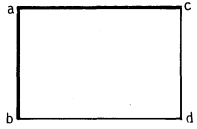
\includegraphics[width=.7\linewidth]{images/ceyhun-204-fig02.png}
		\caption{}\label{Fig:Data2}
	\end{minipage}
	\end{figure} \\
 \figurename \ref{Fig:Data1} \footnote[1]{Since I did not used extra package, I could not create subfigures, then I used figure 1 as a references here and next reference.}Bir tutamaklı yuvarlak ve düzleme serimi. gibi kesilip düzleme serildiğini düşünelim. Yuvarlağın üzerine çizilmeyen çizgelerin bir bölümü, \figurename \ref{Fig:Data1} deki yüzey üzerine
	\begin{figure}[h!]
		\begin{minipage}{0.5\textwidth}
			\centering
			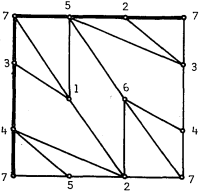
\includegraphics[width=.7\linewidth]{images/ceyhun-204-fig03.png}
			\caption{\hspace{1cm}$D(7)$}\label{Fig:Data3}
		\end{minipage}\hfill
		\begin {minipage}{0.5\textwidth}
		\centering
		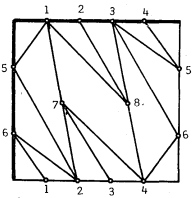
\includegraphics[width=.7\linewidth]{images/ceyhun-204-fig04.png}
		\caption{\hspace{1cm}$I(4,4)$}  \label{Fig:Data4}
	\end{minipage}
	\end{figure} \\
	\figurename \ref{Fig:Data3} \footnote[2]{As I explained footnote1, I used figure3 as reference here} $D(7)$ ve $I(4,4)$ çizgelerinin bir tutamaklı yuvarlağa çizimi.
	
\end{document}